\documentclass[12pt, a4paper]{article}
\usepackage[UTF8]{ctex}
\usepackage{geometry}
\usepackage{graphicx}
\usepackage{amsmath}
\usepackage{float}
\usepackage{caption}
\usepackage{booktabs}
\usepackage{listings}
\usepackage{xcolor}

\geometry{left=2.5cm, right=2.5cm, top=3cm, bottom=3cm}
\setlength{\parindent}{2em}

% 设置图片路径（你自己编译时放图片的文件夹）
\graphicspath{{images/}}

\title{\textbf{数字电子技术课程设计报告}\\ \Large 脉冲波频率检测电路}
\author{\large \textbf{姓名：} [姓名] \quad \textbf{学号：} [学号] \quad \textbf{专业：} 电子信息科学与技术}
\date{2026.6.2}

\begin{document}

\maketitle

\section{设计要求}
本设计要求依靠标准中低规模集成电路搭建脉冲波频率检测电路，我的设计为“定时闸门—计数—锁存—译码显示”四级级联结构。提供精确的 1s 闸门使能信号放行被测脉冲，计数器完成 BCD 码累加，闸门关闭瞬间，触发器捕获并锁存总数，随后清零计数器，进入下一个测量周期。

\begin{figure}[H]
    \centering
    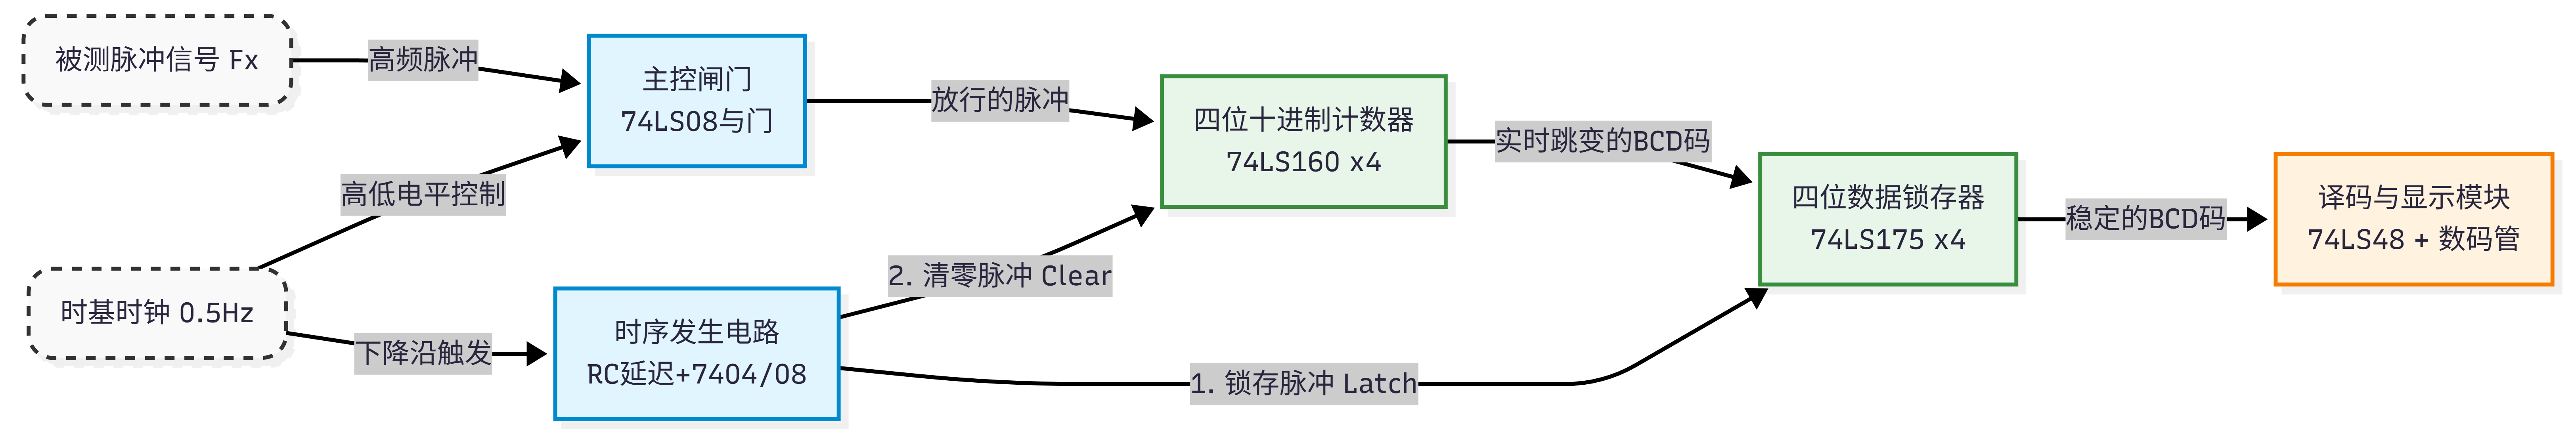
\includegraphics[width=0.8\textwidth]{74LS08 Control Flow with-2026-06-02-053031.png}
    \caption{设计}
\end{figure}

\section{硬件电路设计与参数选型}

\subsection{计数、锁存与显示模块设计}
计数核心选用 4 片 74LS160D 同步十进制计数器，实现最高 9999 Hz 的测量范围。为了保证同步时序，采用同步级联。低位的进位输出端 (RCO) 接入高位的计数使能端 (ENT)，同时所有芯片的时钟端 (CLK) 并行接入被测信号，确保“逢九进一”在同一个时钟上升沿完成。

锁存模块选用 4 片 74LS175D（四 D 触发器）。该模块的必要性在于隔离计数过程的中间态。若无锁存器，数码管将实时显示高速跳变的计数值，超出人眼视觉暂留极限。74LS175 的 D 端接收 160 的状态，仅在 Latch 时钟上升沿到来时，将数据传递至 Q 端。

译码与显示端配置为 74LS48 驱动共阴极七段数码管。LT、BI/RBO等控制脚统一上拉至 5V。

\subsection{时序控制电路}
时序控制电路负责在 1s 闸门关闭的瞬间严格按顺序产生锁存和清零窄脉冲。

最初方案计划选用 74LS123 双单稳态触发器，利用其边沿触发特性级联产生脉冲。但在 Multisim 仿真库中没有找到74123。因此决定采用基础逻辑门（74LS04 非门、74LS08 与门）结合 RC 积分延迟网络，手工搭时序控制电路。

该逻辑电路的工作机制如下：
0.5Hz 的基准时钟下降沿作为触发源。由于 74LS04 具有内部传输延迟，同时在其后级并联 $1\text{k}\Omega$ 电阻与 $1\mu\text{F}$ 电容组成的 RC 网络。当时钟跳变为低电平时，RC 网络按指数规律放电：
\begin{equation}
    V_C(t) = V_{OH} \cdot e^{-\frac{t}{RC}}
\end{equation}
在电容电压降至 TTL 门阈值之前，原信号的反相支路与延迟支路在 74LS08 处发生“逻辑重叠”，从而产生一个宽度 $t_w \approx 0.7RC$ 的高电平尖峰脉冲作为 Latch 信号。随后，利用该 Latch 脉冲的下降沿，驱动第二组 RC 延迟网络，产生滞后约 1ms 的低电平 Clear 脉冲。

\begin{figure}[H]
    \centering
    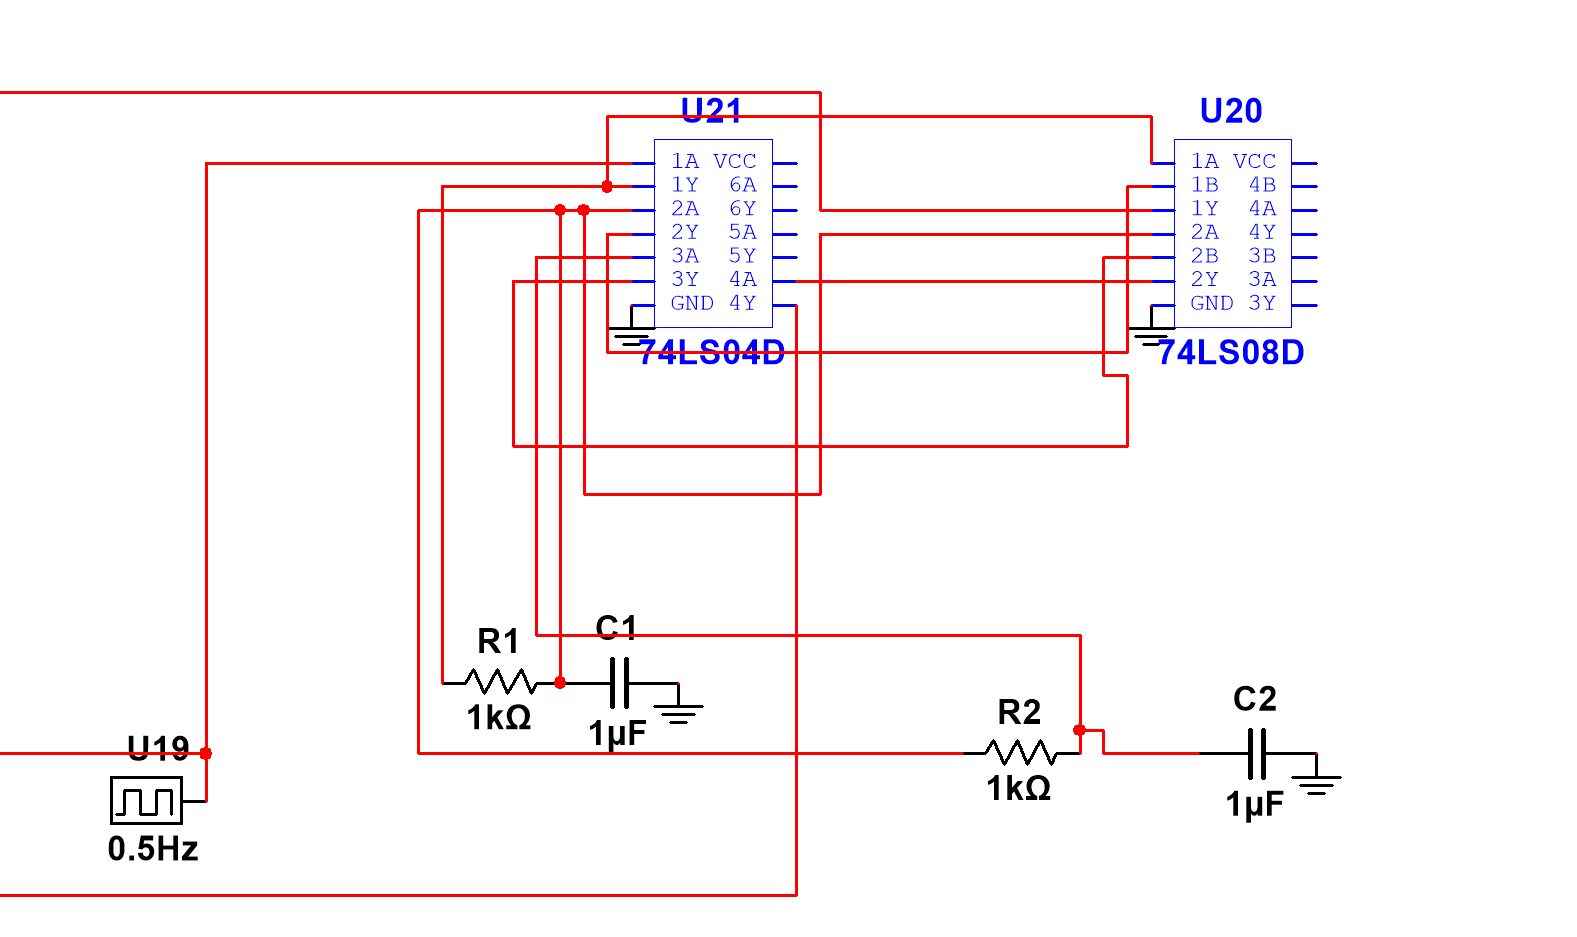
\includegraphics[width=1.0\textwidth]{timing_circuit.png}
    \caption{时序生成电路}
\end{figure}

\section{仿真}
\begin{figure}[H]
    \centering
    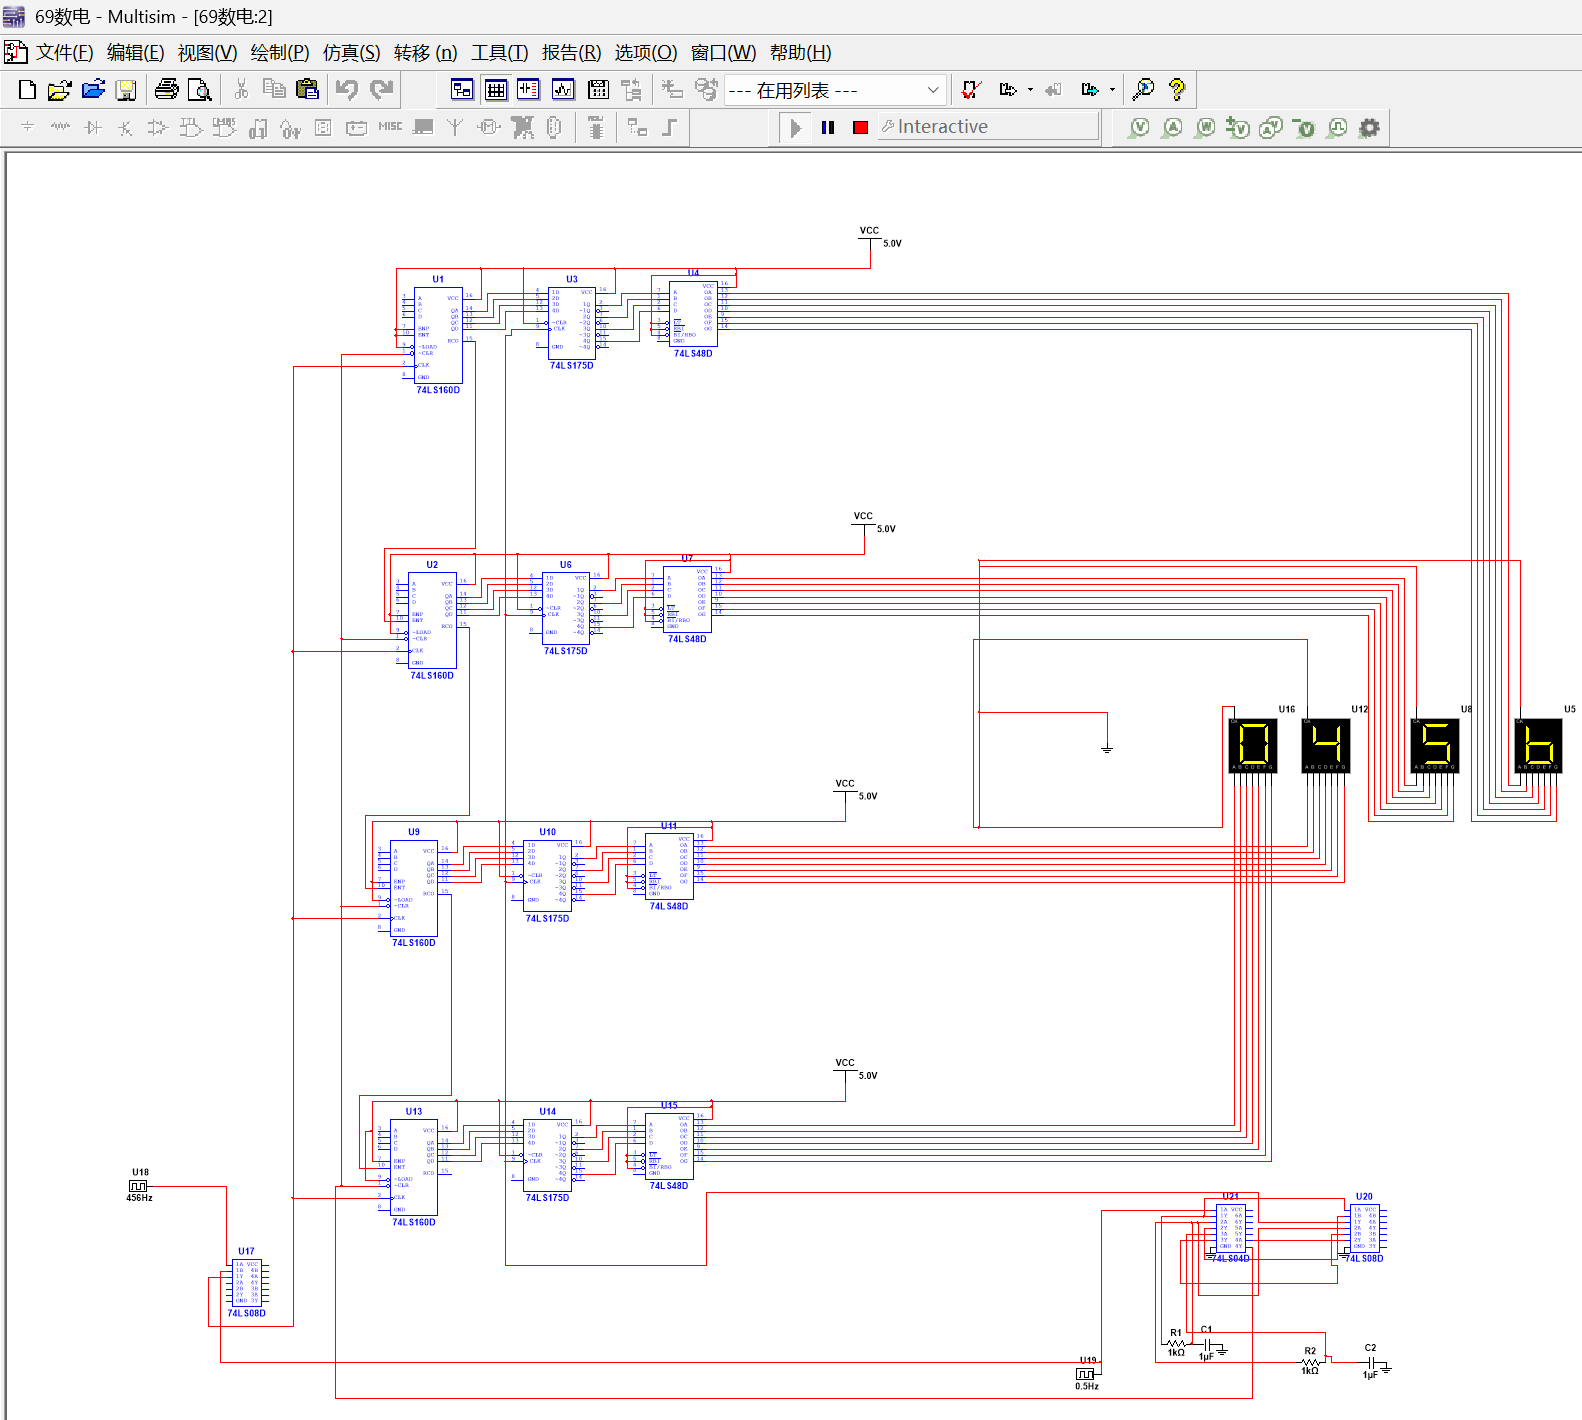
\includegraphics[width=1\textwidth]{full_circuit.png}
    \caption{完整仿真电路}
\end{figure}

\section{仿真}
\begin{figure}[H]
    \centering
    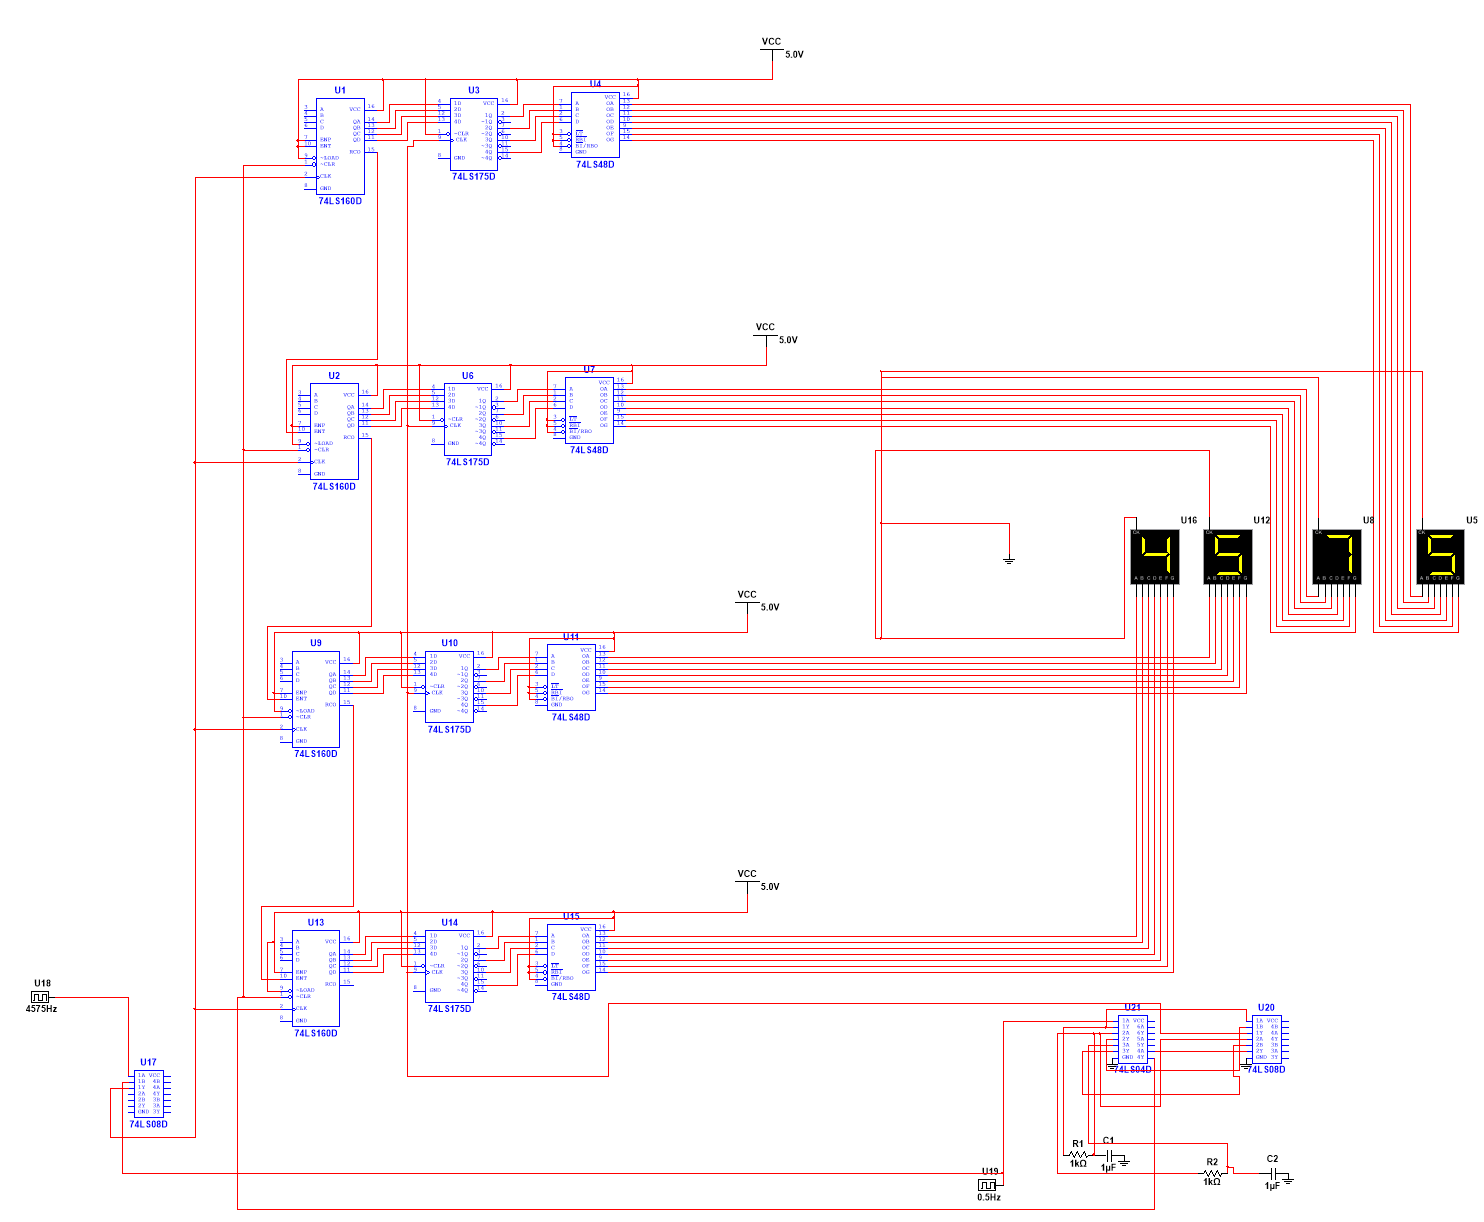
\includegraphics[width=1\textwidth]{0001.png}
    \caption{完整仿真电路(改频率为4575）}
\end{figure}

\section{系统性能评估}
电路对输入脉冲的计数表现出线性与稳定性。在100Hz至9999Hz的动态范围内，数码管能够以 2 秒为一个刷新周期（1 秒计数，1 秒等待），精准输出当前频率对应的十进制数值。

本方案在限定纯硬件数字逻辑的要求内完成任务，优化了级联方式，并通过对门电路传输延迟特性的利用，实现了高稳定性的设计。

\end{document}